\documentclass{article}
\usepackage[T1]{fontenc}
\usepackage{ae,aecompl}

% Ams math
\usepackage{amsmath}
\usepackage{amssymb}

% Figures
\usepackage{graphicx}

\usepackage[letterpaper, margin=1in]{geometry}

\usepackage{hhline}

\graphicspath{img}


\newcommand{\tref}{t_{\textrm{ref}}}

\begin{document}
\def\oddsBasicSinusoidAmplitudeDecayBasicSinusoid{11.1}
\def\errBasicSinusoidAmplitudeDecayBasicSinusoid{4.3}
\def\oddsBasicSinusoidAmplitudeDecayWithTransientBasicSinusoid{271.9}
\def\errBasicSinusoidAmplitudeDecayWithTransientBasicSinusoid{6.8}
\def\oddsBasicSinusoidAmplitudeDecayBasicSinusoidAmplitudeDecayWithTransient{-260.8}
\def\errBasicSinusoidAmplitudeDecayBasicSinusoidAmplitudeDecayWithTransient{5.8}

\title{Preliminary results on fitting to the AMOC data}
\author{Greg Ashton}
\date{}
\maketitle

In this document we show some preliminary results of fitting phenomenological models
to the AMOC data. To select between these phenomenological models we will use the
Bayes factor, defined as
\begin{align}
\mathcal{B}(\textrm{model A}, \textrm{model B}) = \frac{P(\textrm{model A}| \textrm{ data})}{P(\textrm{model B}| \textrm{ data})}
\label{eqn: Bayes}
\end{align}
such that $\mathcal{B} > 1$ provides evidence for model A over model B, while
$\mathcal{B} < 1$ provides evidence for model B over model A. 

We assume the data is a linear sum of the phenomenological model and
gaussian noise to generate a likelihood function for the data. The Bayes factor
is sensitive to both how well the model fits the data, and also the priors chosen
for each model parameter. These priors have been chosen crudely from the data,
and so I will expect the Bayes factors to change when a more expert opinion is
applied.

To fit the models to the data, we have used MCMC simulations which estimate the
posterior distributions for each model parameters. To estimate the marginal
likelihood for each model $P(\textrm{model}| \textrm{ data})$ we have used
so-called `thermodynamic integration', this is a numerical method which has an
associated numerical error which we estimate.

The data that we will consider will be the AMOC flow as a function of the number
of days since the beginning of the data set, 2$^{nd}$ April 2004. In the models a
reference time $\tref$ will be used, we set this to the start of the data set
\begin{align}
\tref = \textrm{2}^{nd}\textrm{ April 2004} = 53097 \textrm{ MJD},
\end{align}
where MJD is the Modified-Julian date.

In the following sections we will introduce each model starting with a
base-model , discuss the fit, and then compare between the models.

\section{Basic sinusoidal `base-model'}

First, let us fit a base-model comprising the sum of a linear function and a
sinusoid
\begin{align}
y(t) = y_0 + \dot{y}_0(t - \tref) + A_0 \sin\left(2\pi \frac{t}{P} + \psi_0\right).
\label{eqn: base-model}
\end{align}
This includes all the basic features which are visible by eye in the data.

As we are using a Bayesian methodology, we need to define priors for each of
the model parameters in Eqn.~\eqref{eqn: base-model} and for $\sigma$, the
gaussian noise in the measurements. These are listed in Table~\ref{tab: base-model}
and were chosen from crude estimates to the data. Note that this choice, for the
base-model parameters, will not produce any bias when compared to modifications
since the priors will cancel out. However, modification model parameters could
produce a bias.
\begin{table}[htb]
\centering
\caption{Prior distributions used in the base-model}
\label{tab: base-model}
\begin{tabular}{lll} \hhline{===}
        Parameter & Distribution &  Units\\ \hline
$y_0$ & Unif(\textrm{-}3.0734, 30.8224) & Sv\\
$y_0$ & $\mathcal{N}$(0, ${1.08}\times 10^{\textrm{-}7}$) & Sv/s\\
$A_0$ & Unif(0, 33.8958) & Sv\\
$P$ & Unif(0, 2.0441) & yrs\\
$\psi_0$ & Unif(0, $2\pi$) & rad\\
$\sigma$ & Unif(0, 33.8958) & Sv\\
\hhline{===}
\end{tabular}
\end{table}

In Fig.~\ref{fig: base-model}A we show the posterior distributions of the
base-model model parameters. This demonstrates that the MCMC simulation has
converged to a solution with gaussian posterior values. In Fig.~\ref{fig: base-model}B
we take the maximum posterior estimate, the MCMC sample with the highest posterior
probability, and plot Eqn.~\eqref{eqn: base-model} with these parameters alongside
the original data.
\begin{figure}[htb]
\centering
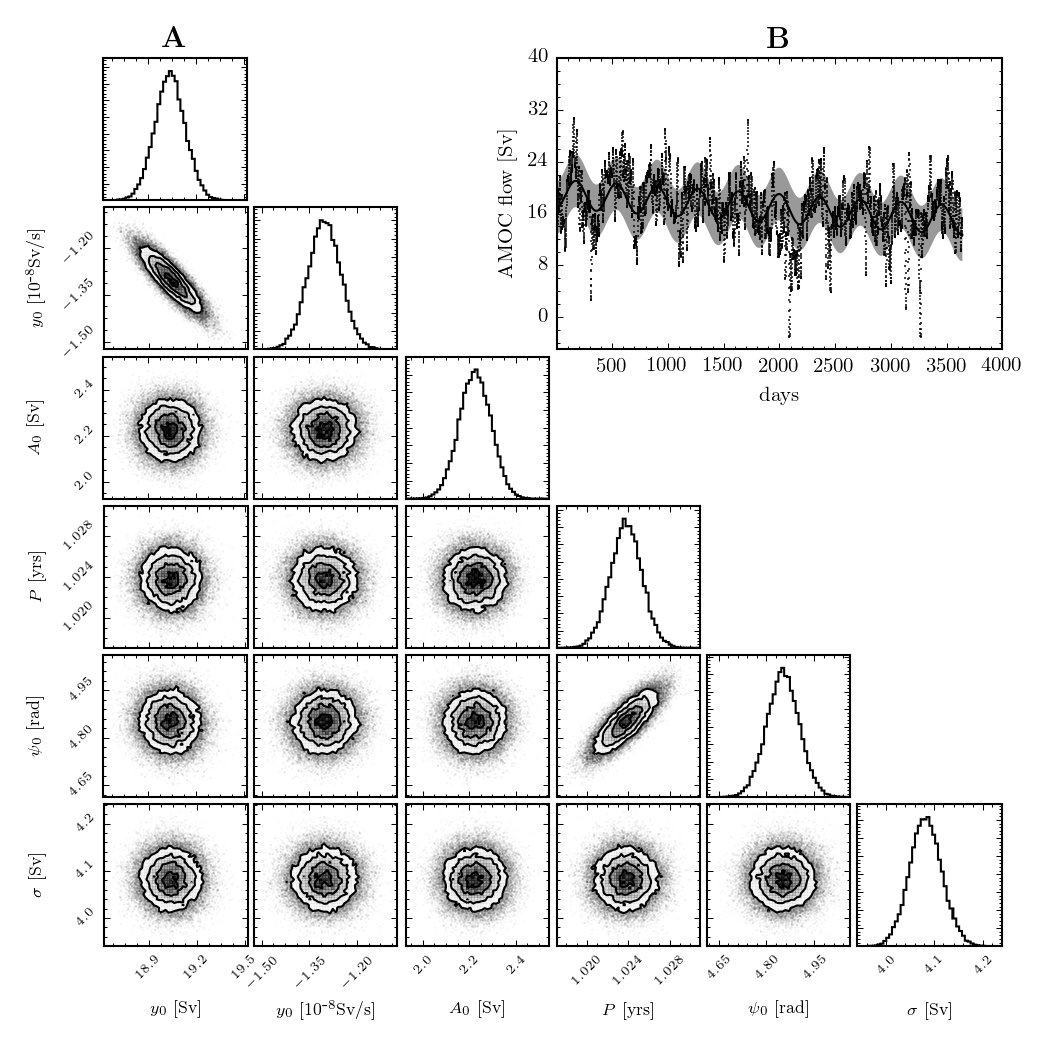
\includegraphics[width=0.8\textwidth]{img/BasicSinusoid_PosteriorWithFit}
\caption{\textbf{A}: Posterior distributions for the model parameters of the
base-model. \textbf{B}: The maximum posterior estimate (MPE) fit to the data.}
\label{fig: base-model}
\end{figure}


\section{Sinusoidal model with evolving amplitude}

The first modification to the base-model we will consider is an evolution of
the sinusoid amplitude.
Specifically, we modify Eqn.~\eqref{eqn: base-model} as follows
\begin{align}
y(t) = y_0 + \dot{y}_0(t - \tref) +
(A_0 + \dot{A}_0(t-\tref)) \sin\left(2\pi \frac{t}{P} + \psi_0\right).
\label{eqn: decay amplitude}
\end{align}
This allows the amplitude to decay $\dot{A} < 0$, or grow $\dot{A} > 0$.

For the priors in this model, we use the same as those in the base-model then
for $\dot{A}$ we use a normal prior with zero mean, giving equal weight to $A$
growing or shrinking, and a standard-deviation of
$0.01\frac{\textrm{range}(y)}{\textrm{range(time)}}$. This is an ad-hoc prior
which will have an effect on the Bayes factor in marginal cases. In Table~\ref{tab: decay amplitude} we list the full set of priors for this model.
\begin{table}[htb]
\centering
\caption{Prior distributions used in the evolving amplitude model}
\label{tab: decay amplitude}
\begin{tabular}{lll} \hhline{===}
        Parameter & Distribution &  Units\\ \hline
$y_0$ & Unif(\textrm{-}3.0734, 30.8224) & Sv\\
$y_0$ & $\mathcal{N}$(0, ${1.08}\times 10^{\textrm{-}7}$) & Sv/s\\
$A_0$ & Unif(0, 33.8958) & Sv\\
$\dot{A}$ & $\mathcal{N}$(0, ${1.08}\times 10^{\textrm{-}9}$) & Sv/s\\
$P$ & Unif(0, 2.0441) & yrs\\
$\psi_0$ & Unif(0, $2\pi$) & rad\\
$\sigma$ & Unif(0, 33.8958) & Sv\\
\hhline{===}
\end{tabular}
\end{table}

In Fig.~\ref{fig: decay amplitude}A we plot the posterior distribution for the
model parameters and in Fig.~\ref{fig: decay amplitude}B we plot the MPE fit to
the data and the data itself.
\begin{figure}[htb]
\centering
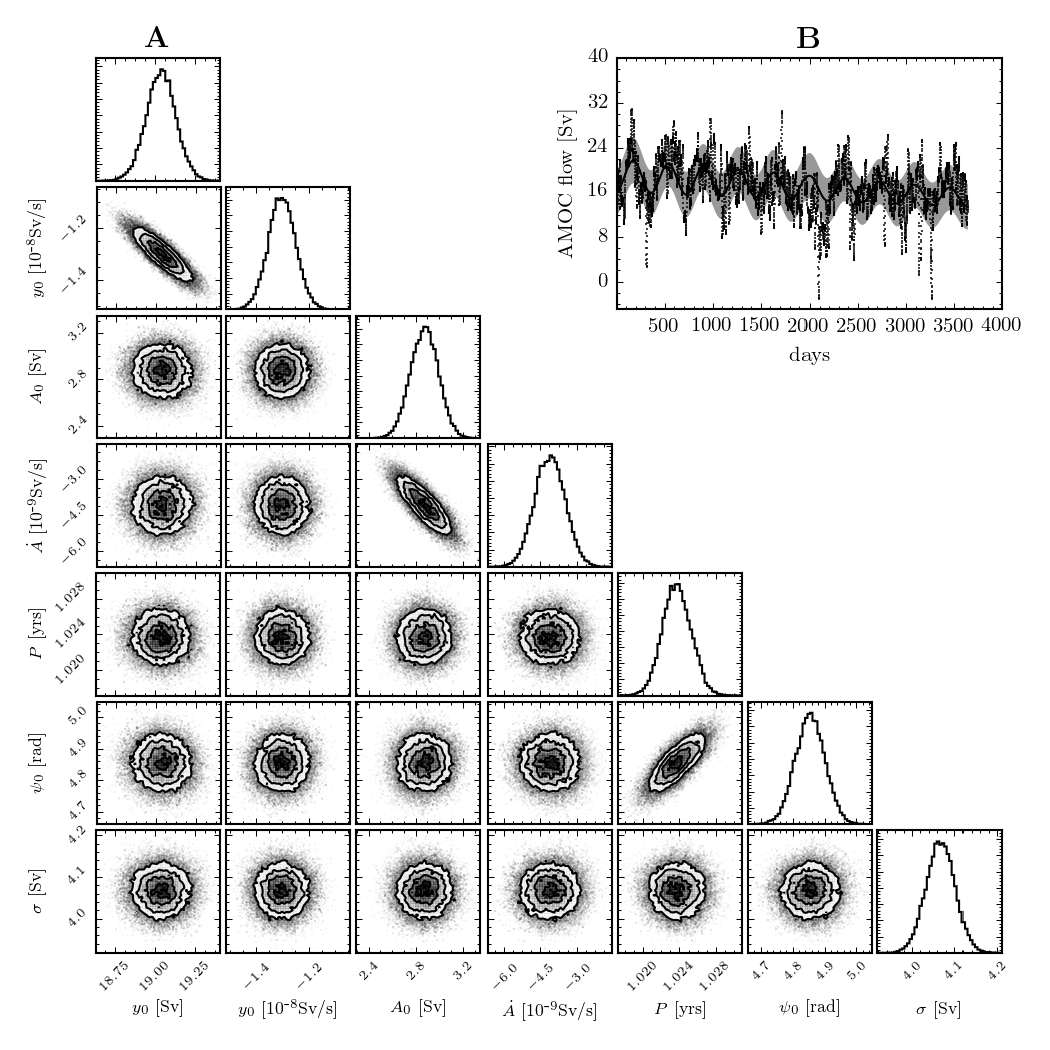
\includegraphics[width=0.8\textwidth]{img/BasicSinusoidAmplitudeDecay_PosteriorWithFit}
\caption{\textbf{A}: Posterior distributions for the model parameters of the
evolving amplitude model. \textbf{B}: The maximum posterior estimate (MPE) fit
to the data.}
\label{fig: decay amplitude}
\end{figure}
From the MPE fit to the data it can be seen that the amplitude is in fact
decaying suggesting that the $\dot{A}$ modification is important. This is
confirmed by looking at its posterior value, we see it is gaussian with a mean
of $\sim-4.5\times10^{-9}$~Sv/s: the amplitude is decaying. Moreover, the
posterior excludes $\dot{A}>0$ indicating that the data is decisive and we have
no uncertainty that the amplitude is decaying. We will comment further on the
potential implications of this in Sec.~\ref{sec: predictions}.

\section{Sinusoidal model with evolving amplitude and transient offset}

The two models considered so far both suffer from poor fitting during the epoch
of 2100~day after the observations start. The data quite clearly does something
unusual at this point, which is around September 2009. Without any physical
input as to what causes this, we can still model it in a simple phenomenological
way. In particular, let us allow the time-averaged AMOC flow ignoring the
secular drift, $y_0$ in the previous models, to undergo a transient period.
That is we let
\begin{align}
y(t) = y_0(t) + \dot{y}_0(t - \tref) + (A_0 + \dot{A}_0(t-\tref)) \sin\left(2\pi \frac{t}{P} + \psi_0\right),
\end{align}
where
\begin{align}
y_0(t) = \left\{
\begin{array}{cl}
y_1^{\textrm{t}} & \textrm{ if } t_1^{\textrm{start}} \le t \le t_1^{\textrm{end}} \\
y_0 & \textrm{ otherwise }
\end{array}
\right..
\label{eqn: transient}
\end{align}

This transient modification introduces three new parameters, the start and end
time of the transient period and the value $y_1^{\textrm{t}}$. For the two times,
we apply a uniform prior limiting them to be within the observation time and
we also add a caveat that $t_1^{\textrm{start}} < t_1^{\textrm{end}}$ to break
the degenerate solutions. For $y_1^\textrm{t}$ we apply the same prior given to
$y_0$ based on a crude estimate to the data. These priors are listed, along with
those for the base-model parameters, in Table~\ref{tab: decay amplitude transient}.
\begin{table}[htb]
\centering
\caption{Prior distributions used in the evolving amplitude model with a transient offset}
\label{tab: decay amplitude transient}
\begin{tabular}{lll} \hhline{===}
        Parameter & Distribution &  Units\\ \hline
$y_0$ & Unif(\textrm{-}3.0734, 30.8224) & Sv\\
$y_0$ & $\mathcal{N}$(0, ${1.08}\times 10^{\textrm{-}7}$) & Sv/s\\
$A_0$ & Unif(0, 33.8958) & Sv\\
$\dot{A}$ & $\mathcal{N}$(0, ${1.08}\times 10^{\textrm{-}9}$) & Sv/s\\
$y_1$
 & Unif(0, 33.8958) & Sv\\
$t_1^\mathrm{start}$
 & Unif(0, 3642) & days\\
$t_1^\mathrm{end}$
 & Unif(0, 3642) & days\\
$P$ & Unif(0, 2.0441) & yrs\\
$\psi_0$ & Unif(0, $2\pi$) & rad\\
$\sigma$ & Unif(0, 33.8958) & Sv\\
\hhline{===}
\end{tabular}
\end{table}

In Fig.~\ref{fig: decay amplitude transient}A we show the posterior values and
in Fig.~\ref{fig: decay amplitude transient}B we show the MPE fit for the evolving
amplitude with a transient offset model.
\begin{figure}[htb]
\centering
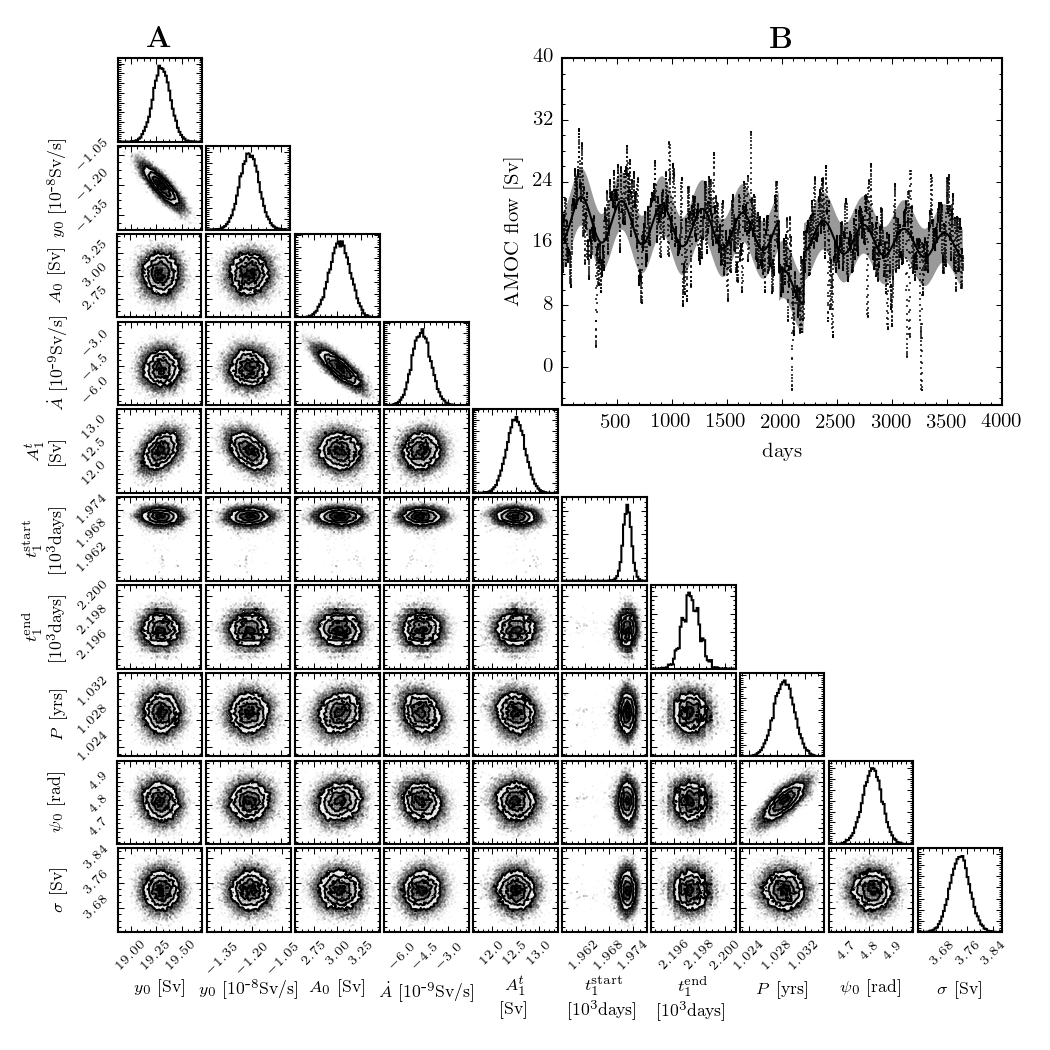
\includegraphics[width=0.8\textwidth]{img/BasicSinusoidAmplitudeDecayWithTransient_PosteriorWithFit}
\caption{\textbf{A}: Posterior distributions for the model parameters of the
evolving amplitude with transient offset model. \textbf{B}: The maximum posterior estimate (MPE) fit
to the data.}
\label{fig: decay amplitude transient}
\end{figure}
This clearly demonstrates that the transient modification introduced in
Eqn.~\eqref{eqn: transient} captures the deviations shown in the data. This modification
makes little change to the posterior values of the other model parameters except
for $y_0$ and $\dot{y}_0$ which is to be expected. In the next section we will
compare between the three models, and then attempt to interpret the model in
the last section.

\section{Bayes factor comparisons}
In this section we will compare between the three models. This can easily be
done quantitatively by calculating the Bayes factor defined in Eqn,~\eqref{eqn: Bayes}.
In Table~\ref{tab: bayes factors} we present the Bayes factor being the probability
of model~A over model~B; a Bayes factor greater than 1 indicates a preference for
model~A over model~B.
\begin{table}[htb]
\centering
\caption{Bayes factors between the models compared in this work}
\label{tab: bayes factors}
\begin{tabular}{ccc} \hhline{===}
model A & model B & $\log_{10}(\mathcal{B}(\textrm{model A}, \textrm{model B}))$\\ \hline
evolution of the amplitude & base-model &
$ \oddsBasicSinusoidAmplitudeDecayBasicSinusoid \pm
  \errBasicSinusoidAmplitudeDecayBasicSinusoid$\\
evolution of the amplitude with transient & base-model &
$ \oddsBasicSinusoidAmplitudeDecayWithTransientBasicSinusoid \pm
  \errBasicSinusoidAmplitudeDecayWithTransientBasicSinusoid$ \\
evolution of the amplitude with transient & evolution of the amplitude &
$ \oddsBasicSinusoidAmplitudeDecayWithTransientBasicSinusoidAmplitudeDecay \pm
  \errBasicSinusoidAmplitudeDecayWithTransientBasicSinusoidAmplitudeDecay$
\end{tabular}
\end{table}
From this table we confirm what is already evident from the MPE fits to the
data: the evolution of the amplitude model is a significant improvement over
the base-model and the inclusion of a transient offset is an improvement again
over the evolution of the amplitude model.

At this time, I do not have a clear idea of why this transient occurs or how it
is relevant to the problem in hand. However, if it is to be treated as an
abnormality and we wish to discuss the behaviour of the solution in the region
outside of the transient, it is proper to use the posterior parameters
estimated from this model, since we understand how they are contaminated by the
transient region.

\section{Predicting the amplitude decay}
\label{sec: predictions}

The decay of the amplitude, if it persists into the future, means that eventually
the oscillations of the AMOC flow may become smaller than our resolution to
measure it. When this happens can be estimated from the posteriors, taking
typical values we see that
\begin{align}
\dot{A} \approx -4.5\times10^{-9}\textrm{ Sv/s}
\end{align}
In order to estimate how long it will take for this to be smaller than the
some threshold $\sigma_A$, we define $t^{*}$ as the point where the sinusoid amplitude
variations are equal to the threshold
\begin{align}
 & A_0 + \dot{A}_0(t^{*} - \tref) = \sigma_A  \\
\Rightarrow \hspace{5mm}  & t^{*}   = \tref + \frac{\sigma_A - A_0}{\dot{A}}
\end{align}
Taking $\sigma_A = 0.1$ this predicts that the condition is met approximately
7500 days after $\tref$, which is MJD~60555, or the $9^{th}$ of September 2024.





\end{document}
